\section{The Dataset}\label{sec:dataset}
\subsection{Data Generation}
\subsection{Data Scaling and Transformations}
\section{Performance Metrics}\label{seq:perf_metrics}
\section{Results}\label{sec:results}
\subsection{Benchmarks of Hyperparameters}\label{subsec:benchmarks}
\subsubsection{Baseline Model}
\subsubsection{Pretraining}
\subsubsection{Burn-in length}
\subsubsection{Number of model parameters}

\subsection{Neutralino-Neutralino Cross Sections}\label{subsec:neuralino_experiments}

\begin{table}[h!]
    \centering
\begin{tabular}{c@{\hspace{1cm}}c@{\hspace{1cm}}c@{\hspace{1cm}}c@{\hspace{1cm}}c@{\hspace{1cm}}c}
\hline
    Burn-in steps & \makecell{Number \\of \\steps between} & Kernel & \makecell{Number \\ of \\ results} & \makecell{Pretraining \\ epochs} & \makecell{Pretraining \\ batch size} \\
\hline
    2500 & 10 & NUTS & 1000 & 1000 & 32 \\
\hline
\end{tabular}
\caption{
    The table shows the training configuration used to sample the models listed in table~\ref{tab:deep_models}.
}
\label{tab:NN_mse_scores}
\end{table}


\begin{table}[h!]
    \centering
\begin{tabular}{c@{\hspace{1cm}}c@{\hspace{1cm}} c}
\hline
      Model number & Architechture & Number of parameters \\
\hline
    1 & 5-50-1 & 351\\
    2 & 5-50-50-1 & 2901\\
    3 & 5-50-50-50-1 & 5451\\
    4 & 5-50-50-50-50-1 & 8001\\
    5 & 5-50-50-50-50-50-1 & 10551\\
\hline
\end{tabular}
\caption{
    The table shows the models used in this section. For each model, 1000 sampled networks are used to
    generate each result shown in this section. The architecture describe number of nodes per layer.
    For each hidden layer, the same activation function is used. The final layer uses an identity function.
}
\label{tab:deep_models}
\end{table}

\begin{figure}
    \centering
    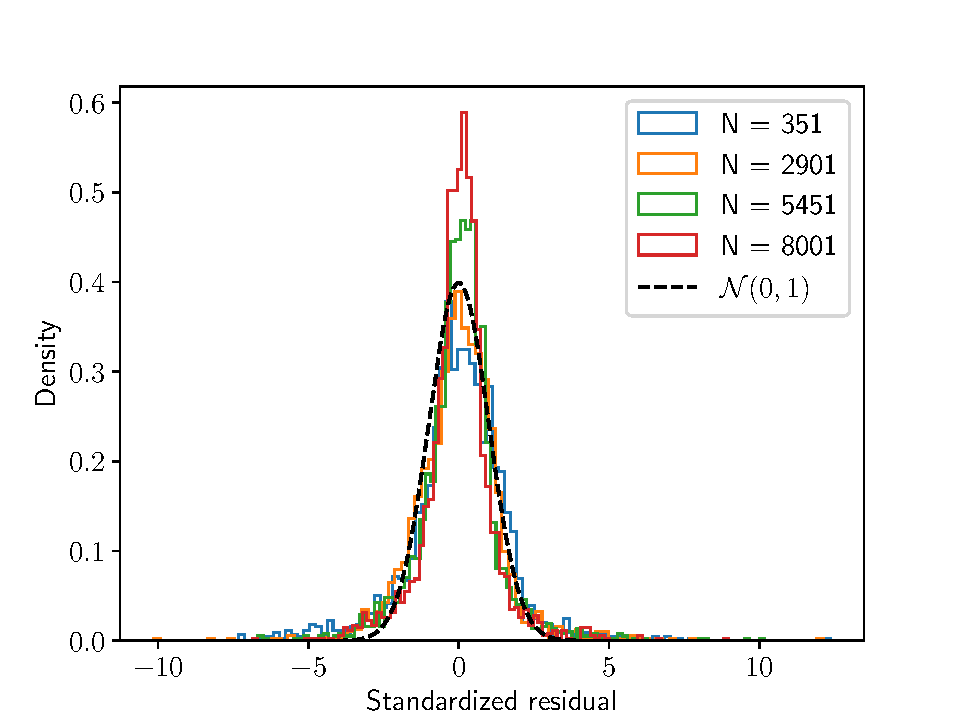
\includegraphics[scale=1]{figures/standardized_residuals/standardized_residual_simple_models.pdf}
    \caption{The figure shows histograms of the standardized residuals computed for 
        different BNNs. The normal distribution is drawn as dotted line. 
    }
    \label{fig:standardized_residual}
\end{figure}
